\documentclass[11pt,a4paper]{article}
\usepackage[margin=1in]{geometry}
\usepackage{amsmath,amssymb,booktabs,array,longtable,hyperref,xcolor}
\usepackage{tikz}
\usepackage{caption,subcaption}
\usepackage{graphicx}
\usepackage{multirow}

% TikZ setup for Feynman diagrams
\pgfdeclarelayer{nodelayer}
\pgfdeclarelayer{edgelayer}
\pgfsetlayers{edgelayer,nodelayer,main}
\tikzstyle{straight}=[-, draw=black, thick]
\tikzstyle{wavy}=[-, draw=black, thick, decorate,
  decoration={snake, amplitude=1.2pt, segment length=5pt}]
\tikzstyle{none}=[]

\title{Multi-Pair Electron--Positron Production in Muon Decay:\\
Experimental Frontier from Diagram Enumeration and NDA}
\author{Tony Menzo and Claude Opus 4.6 (high effort)\\[4pt]
\small Computed with \textsc{Heptapod}}
\date{\today}

\begin{document}
\maketitle

\begin{abstract}
We systematically study the Standard Model decay
$\mu^+ \to \bar\nu_\mu \nu_e \, e^+ + n(e^+e^-)$ for
$n = 0, 1, 2, 3$ electron--positron pairs.
Using automated tree-level diagram enumeration, naive dimensional analysis
(NDA), and exact MadGraph calculations, we determine the branching ratio
as a function of the pair multiplicity~$n$.
The number of contributing Feynman diagrams grows from~1 at $n=0$
to~149{,}400 at $n=3$, yet the rate is dominated at every multiplicity
by diagrams with a single heavy $W$ propagator.
MadGraph cross-checks at $n=1$ and $n=2$ validate the NDA estimates
to within a factor of a few, confirming
$\text{BR}(n\!=\!1) = 3.56\times10^{-5}$ and
$\text{BR}(n\!=\!2) = 4.34\times10^{-10}$.
The effective per-pair suppression factor is approximately
$(\alpha/\pi)^2 \approx 5\times10^{-6}$, modulated by a rapidly growing
diagram multiplicity that partially compensates the phase-space penalty.
We identify $n = 3$ (BR $\sim 10^{-13}$) as the experimental frontier
for Mu3e Phase~I, and $n = 4$ (BR $\sim 10^{-16}$) as marginally
accessible at Mu3e Phase~II.
\end{abstract}

%---------------------------------------------------------------------
\section{Introduction}
\label{sec:intro}
%---------------------------------------------------------------------

The dominant decay of the muon,
$\mu^+ \to e^+ \nu_e \bar\nu_\mu$, proceeds through a single
$W$ boson exchange with unit branching ratio.
Higher-multiplicity variants in which one or more virtual photons
radiated from the charged lepton lines convert into
$e^+e^-$ pairs provide a clean probe of higher-order electroweak
dynamics.
The $n=1$ channel,
$\mu^+ \to e^+e^+e^- \nu_e \bar\nu_\mu$,
was measured by SINDRUM~\cite{sindrum} at
$\text{BR} = (3.4 \pm 0.4)\times10^{-5}$,
and NLO corrections have been computed~\cite{pruna,fael}.
The $n=2$ channel (seven-body) has been predicted at
$\text{BR} = (3.93 \pm 0.01)\times10^{-10}$ by
Hostert \textit{et al.}~\cite{hostert} and is expected to be
first observed at Mu3e Phase~I with $\sim\!1{,}000$ events.
No prediction exists for $n \geq 3$.

The question we address is: \emph{what is the largest $n$ for which
$\mu^+ \to \bar\nu_\mu \nu_e \, e^+ + n(e^+e^-)$ remains
experimentally observable?}
The answer is determined by the interplay between the per-pair
suppression (coupling, phase space, propagator) and the combinatorial
explosion of contributing Feynman diagrams.

\paragraph{Experimental landscape.}
The relevant current and planned muon experiments are:
\begin{itemize}
\item \textbf{SINDRUM (1985)}: Measured $\text{BR}(n\!=\!1)$ from
  $7.3\times10^{12}$ stopped muons. Sensitivity $\sim\!10^{-5}$.
\item \textbf{Mu3e Phase~I} (PSI, 2025--2026):
  $10^8\;\mu^+$/s on the $\pi$E5 beamline,
  $2.5\times10^{15}$ total stops,
  single-event sensitivity (SES) $= 2\times10^{-15}$.
\item \textbf{Mu3e Phase~II} (PSI, $\sim$2030):
  $10^9\;\mu^+$/s with the HiMB upgrade,
  $5.5\times10^{16}$ total stops, SES $\sim 10^{-16}$.
\item \textbf{HiMB future}: Up to $10^{10}\;\mu^+$/s,
  pushing the BR floor toward $\sim\!10^{-18}$.
\end{itemize}

%---------------------------------------------------------------------
\section{Method}
\label{sec:method}
%---------------------------------------------------------------------

Our analysis pipeline combines three complementary tools:

\paragraph{Diagram enumeration.}
\textsc{FeynGraph} enumerates all tree-level Feynman diagrams for a
given process and classifies them by the number of heavy
($W$, $Z$) propagators.
Each additional heavy propagator introduces a suppression
$(m_\mu/M_W)^4 \sim 10^{-13}$, establishing a clear hierarchy
among diagram classes.

\paragraph{Naive dimensional analysis (NDA).}
For each diagram class, NDA estimates the partial width from the
coupling structure, propagator masses, and $n$-body phase-space volume
$\Phi_n$.
The massless $n$-body phase space scales as
\begin{equation}
\Phi_n = \frac{M^{2n-4}}{2^{4n-5}\,\pi^{2n-3}\,(n-1)!\,(n-2)!}\,,
\label{eq:phasespace}
\end{equation}
where $M = m_\mu$ is the mother particle mass.

\paragraph{MadGraph.}
Exact tree-level widths are computed with MadGraph5\_aMC@NLO using the
\texttt{sm-lepton\_masses} model (which retains $m_\mu, m_e \neq 0$).
Coupling-order restrictions (\texttt{QED$\leq$4}, \texttt{QED$\leq$6})
isolate the dominant diagram class for independent cross-checking.

%---------------------------------------------------------------------
\section{Results}
\label{sec:results}
%---------------------------------------------------------------------

\subsection{Diagram enumeration}
\label{sec:diagrams}

Table~\ref{tab:diagrams} summarizes the diagram enumeration for each
multiplicity.
The total number of Feynman diagrams grows super-exponentially:
$1 \to 18 \to 1{,}122 \to 149{,}400$ from $n=0$ to $n=3$, driven
by the combinatorial ways of attaching photon propagators to the
increasing number of charged lines.

\begin{table}[h]
\centering
\caption{Tree-level Feynman diagram count by heavy-propagator class
for $\mu^+ \to \bar\nu_\mu\nu_e\,e^+ + n(e^+e^-)$.
The dominant class (fewest heavy propagators) is highlighted.}
\label{tab:diagrams}
\begin{tabular}{cccccccccc}
\toprule
$n$ & Particles & \multicolumn{7}{c}{Diagrams by heavy-propagator count}
    & Total \\
\cmidrule(lr){3-9}
    &           & 1$W$ & 2$W$ & 3$W$ & 4$W$ & 5$W$ & 6$W$ & 7$W$ & \\
\midrule
0 & 3  & \textbf{1} & -- & -- & -- & -- & -- & -- & 1 \\
1 & 5  & \textbf{4} & 12 & 2  & -- & -- & -- & -- & 18 \\
2 & 7  & \textbf{84} & 378 & 504 & 138 & 18 & -- & -- & 1{,}122 \\
3 & 9  & \textbf{4{,}320} & 24{,}768 & 52{,}272 & 47{,}520 & 16{,}416 & 3{,}744 & 360 & 149{,}400 \\
\bottomrule
\end{tabular}
\end{table}

The dominant-class fraction shrinks rapidly:
100\% at $n=0$, 22\% at $n=1$, 7.5\% at $n=2$, and 2.9\% at $n=3$.
Yet the subleading classes are suppressed by
$(m_\mu/M_W)^4 \sim 10^{-13}$ per additional heavy propagator in the
rate, so they contribute negligibly to the total width at every~$n$.

Figure~\ref{fig:diagrams} shows representative dominant-class diagrams.
At each multiplicity, the dominant topology consists of a single $W$
exchange (the Michel vertex) dressed by $n$~virtual photons that
each convert to an $e^+e^-$ pair.
The couplings for the dominant class are
$g_w^2 \, e^{2n}$, confirming the purely electromagnetic character
of the additional pair production.

\begin{figure}[h]
\centering
\begin{subfigure}[b]{0.28\textwidth}
\centering
\begin{tikzpicture}[scale=0.35]
    \begin{pgfonlayer}{nodelayer}
        \node [style = none] (0) at (0, 5) {\tiny $\mu^+$};
        \node [style = none] (1) at (3.5, 4) {};
        \node [style = none] (2) at (10, 5) {\tiny $e^+$};
        \node [style = none] (3) at (6.5, 6) {};
        \node [style = none] (4) at (6.7, 9.7) {\tiny $\nu_e$};
        \node [style = none] (5) at (3.3, 0.3) {\tiny $\bar\nu_\mu$};
    \end{pgfonlayer}
    \begin{pgfonlayer}{edgelayer}
        \draw[style=straight] (1.center) to (0.center);
        \draw[style=straight] (3.center) to (2.center);
        \draw[style=straight] (4.center) to (3.center);
        \draw[style=straight] (1.center) to (5.center);
        \draw[style=wavy] (1.center) to (3.center);
    \end{pgfonlayer}
\end{tikzpicture}
\caption*{$n=0$: 1~diagram}
\end{subfigure}
\hfill
\begin{subfigure}[b]{0.33\textwidth}
\centering
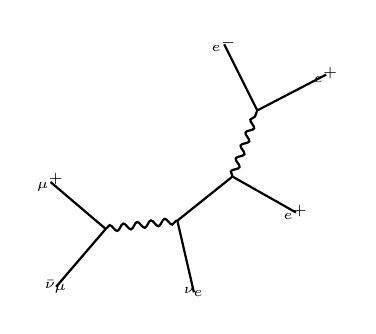
\begin{tikzpicture}[scale=0.35]
    \begin{pgfonlayer}{nodelayer}
        \node [style = none] (0) at (0, 4.5) {\tiny $\mu^+$};
        \node [style = none] (1) at (2, 2.8) {};
        \node [style = none] (2) at (8.9, 3.4) {\tiny $e^+$};
        \node [style = none] (3) at (6.6, 4.7) {};
        \node [style = none] (4) at (10, 8.4) {\tiny $e^+$};
        \node [style = none] (5) at (7.5, 7.1) {};
        \node [style = none] (6) at (6.3, 9.5) {\tiny $e^-$};
        \node [style = none] (7) at (5.2, 0.5) {\tiny $\nu_e$};
        \node [style = none] (8) at (4.6, 3.1) {};
        \node [style = none] (9) at (0.2, 0.7) {\tiny $\bar\nu_\mu$};
    \end{pgfonlayer}
    \begin{pgfonlayer}{edgelayer}
        \draw[style=straight] (1.center) to (0.center);
        \draw[style=straight] (3.center) to (2.center);
        \draw[style=straight] (5.center) to (4.center);
        \draw[style=straight] (6.center) to (5.center);
        \draw[style=straight] (7.center) to (8.center);
        \draw[style=straight] (1.center) to (9.center);
        \draw[style=wavy] (1.center) to (8.center);
        \draw[style=straight] (3.center) to (8.center);
        \draw[style=wavy] (3.center) to (5.center);
    \end{pgfonlayer}
\end{tikzpicture}
\caption*{$n=1$: 4~diagrams}
\end{subfigure}
\hfill
\begin{subfigure}[b]{0.35\textwidth}
\centering
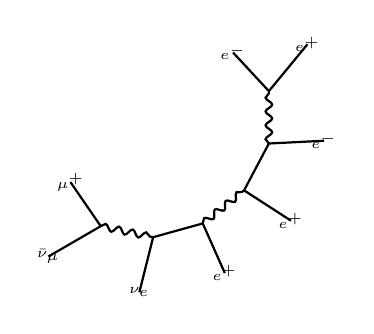
\begin{tikzpicture}[scale=0.35]
    \begin{pgfonlayer}{nodelayer}
        \node [style = none] (0) at (0.8, 4.5) {\tiny $\mu^+$};
        \node [style = none] (1) at (1.9, 2.9) {};
        \node [style = none] (2) at (6.4, 1.2) {\tiny $e^+$};
        \node [style = none] (3) at (5.6, 3.0) {};
        \node [style = none] (4) at (8.8, 3.1) {\tiny $e^+$};
        \node [style = none] (5) at (7.1, 4.2) {};
        \node [style = none] (6) at (9.4, 9.5) {\tiny $e^+$};
        \node [style = none] (7) at (8.0, 7.8) {};
        \node [style = none] (8) at (10, 6.0) {\tiny $e^-$};
        \node [style = none] (9) at (8.0, 5.9) {};
        \node [style = none] (10) at (6.7, 9.2) {\tiny $e^-$};
        \node [style = none] (11) at (3.3, 0.5) {\tiny $\nu_e$};
        \node [style = none] (12) at (3.8, 2.5) {};
        \node [style = none] (13) at (0, 1.8) {\tiny $\bar\nu_\mu$};
    \end{pgfonlayer}
    \begin{pgfonlayer}{edgelayer}
        \draw[style=straight] (1.center) to (0.center);
        \draw[style=straight] (3.center) to (2.center);
        \draw[style=straight] (5.center) to (4.center);
        \draw[style=straight] (7.center) to (6.center);
        \draw[style=straight] (8.center) to (9.center);
        \draw[style=straight] (10.center) to (7.center);
        \draw[style=straight] (11.center) to (12.center);
        \draw[style=straight] (1.center) to (13.center);
        \draw[style=wavy] (1.center) to (12.center);
        \draw[style=straight] (3.center) to (12.center);
        \draw[style=wavy] (3.center) to (5.center);
        \draw[style=straight] (5.center) to (9.center);
        \draw[style=wavy] (9.center) to (7.center);
    \end{pgfonlayer}
\end{tikzpicture}
\caption*{$n=2$: 84~diagrams}
\end{subfigure}
\caption{Representative dominant-class (single-$W$) Feynman diagrams for
$n = 0, 1, 2$ electron--positron pairs.
Each additional pair arises from a virtual photon (wavy line) radiated
off an existing charged-fermion line.
The dominant-class diagram count and coupling structure
($g_w^2 e^{2n}$) are indicated.}
\label{fig:diagrams}
\end{figure}


\subsection{NDA branching ratio estimates}
\label{sec:nda}

Table~\ref{tab:nda} presents the NDA branching ratio estimates for
each multiplicity and diagram class.
In every case, the single-$W$ class overwhelmingly dominates, with
subleading classes suppressed by at least $10^{13}$ per additional
heavy propagator.

\begin{table}[h]
\centering
\caption{NDA partial widths and branching ratios for the dominant
(1$W$) class at each pair multiplicity.
The NDA formula, number of diagrams, width per diagram, total class
width, and branching ratio are shown.
The reference total width is
$\Gamma_\mu = 2.996\times10^{-19}$~GeV.}
\label{tab:nda}
\begin{tabular}{cclccc}
\toprule
$n$ & Diagrams & NDA formula & Width/diag (GeV) & Total width (GeV) & BR \\
\midrule
0 & 1
  & $\dfrac{g_w^4\, M^5}{64\pi^3\, M_W^4}$
  & $8.56\times10^{-19}$ & $8.56\times10^{-19}$ & $2.86$ \\[8pt]
1 & 4
  & $\dfrac{g_w^4\, e^4\, M^5}{\pi^7\, M_W^4}$
  & $1.39\times10^{-24}$ & $5.55\times10^{-24}$ & $1.85\times10^{-5}$ \\[8pt]
2 & 84
  & $\dfrac{g_w^4\, e^8\, M^5}{\pi^{11}\, M_W^4}$
  & $6.73\times10^{-30}$ & $5.65\times10^{-28}$ & $1.89\times10^{-9}$ \\[8pt]
3 & 4{,}320
  & $\dfrac{g_w^4\, e^{12}\, M^5}{\pi^{15}\, M_W^4}$
  & $5.73\times10^{-35}$ & $2.47\times10^{-31}$ & $8.26\times10^{-13}$ \\
\bottomrule
\end{tabular}
\end{table}

The NDA estimate at $n=0$ gives $\text{BR} = 2.86$, an $O(1)$ number
consistent with the known result (the Michel decay saturates the total
width).
The NDA accuracy is typical: correct to within a factor of a few at each
multiplicity, as confirmed by MadGraph in the following section.


\subsection{MadGraph cross-checks}
\label{sec:madgraph}

Table~\ref{tab:madgraph} compares NDA and MadGraph results for
$n = 1$ and $n = 2$.
In both cases, restricting MadGraph to the dominant coupling order
(\texttt{QED$\leq$4} for $n=1$, \texttt{QED$\leq$6} for $n=2$)
reproduces the full result, confirming that subleading diagram classes
are negligible.

\begin{table}[h]
\centering
\caption{Comparison of NDA estimates with exact MadGraph tree-level
widths for the dominant diagram class.}
\label{tab:madgraph}
\begin{tabular}{cccccc}
\toprule
$n$ & NDA width (GeV) & MG width (GeV) & NDA BR & MG BR & Ratio \\
\midrule
1 & $5.55\times10^{-24}$ & $1.066\times10^{-23}$ & $1.85\times10^{-5}$ & $3.56\times10^{-5}$ & 0.52 \\
2 & $5.65\times10^{-28}$ & $1.301\times10^{-28}$ & $1.89\times10^{-9}$ & $4.34\times10^{-10}$ & 4.3 \\
\bottomrule
\end{tabular}
\end{table}

Key observations:
\begin{itemize}
\item At $n=1$, the MadGraph result
  $\text{BR} = 3.56\times10^{-5}$ agrees with the SINDRUM measurement
  $(3.4 \pm 0.4)\times10^{-5}$ to within one sigma.
\item At $n=2$, MadGraph gives
  $\text{BR} = 4.34\times10^{-10}$, consistent with the prediction
  of $(3.93 \pm 0.01)\times10^{-10}$ from Ref.~\cite{hostert}.
\item The NDA-to-MadGraph ratio varies from 0.52 to 4.3, typical of
  NDA accuracy.
  At $n=1$, NDA underestimates by a factor of~2; at $n=2$, it
  overestimates by a factor of~4.
  This variation reflects the growing importance of destructive
  interference among diagrams at higher multiplicity, which NDA
  does not capture.
\end{itemize}


%---------------------------------------------------------------------
\section{Per-pair suppression factor}
\label{sec:suppression}
%---------------------------------------------------------------------

The effective branching ratio suppression per additional $e^+e^-$ pair
results from the competition of three factors:

\paragraph{Coupling.}
Each pair introduces two QED vertices (photon emission and
$\gamma \to e^+e^-$ conversion), contributing a factor
$e^4 = (4\pi\alpha)^2 \approx 8.4\times10^{-3}$
to $|\mathcal{M}|^2$.

\paragraph{Phase space.}
Adding two massless particles to a $k$-body final state multiplies
the phase-space volume by
\begin{equation}
\frac{\Phi_{k+2}}{\Phi_k}
= \frac{m_\mu^4}{256\,\pi^4 \cdot k(k\!+\!1)(k\!-\!1)(k\!-\!2)!/(k\!-\!2)!}\,,
\label{eq:phi_ratio}
\end{equation}
which ranges from $6.9\times10^{-11}$
($k = 3 \to 5$) to $2.1\times10^{-12}$ ($k = 7 \to 9$).
The phase-space penalty increases with multiplicity because the
available energy must be shared among more particles.

\paragraph{Diagram multiplicity.}
The number of dominant-class diagrams grows as
$1 \to 4 \to 84 \to 4{,}320$ (ratios: $4, 21, 51$), partially
compensating the coupling and phase-space suppression.
Each new pair can attach its photon to any of the existing charged
lines, and the identical-particle permutations multiply rapidly.

\medskip
The net per-pair suppression factors are:

\begin{table}[h]
\centering
\caption{Per-pair suppression factor
$\text{BR}(n\!+\!1)/\text{BR}(n)$ from NDA, MadGraph, and analytical
estimates.}
\label{tab:suppression}
\begin{tabular}{lccc}
\toprule
Transition & NDA & MadGraph & $(\alpha/\pi)^2$ \\
\midrule
$n\!=\!0 \to 1$ & $6.5\times10^{-6}$ & $3.6\times10^{-5}$ & $5.4\times10^{-6}$ \\
$n\!=\!1 \to 2$ & $1.0\times10^{-4}$ & $1.2\times10^{-5}$ & $5.4\times10^{-6}$ \\
$n\!=\!2 \to 3$ & $4.4\times10^{-4}$ & -- & $5.4\times10^{-6}$ \\
\bottomrule
\end{tabular}
\end{table}

The NDA per-pair suppression weakens with each step (from
$6.5\times10^{-6}$ to $4.4\times10^{-4}$) because the diagram
multiplicity growth outpaces the additional phase-space penalty.
The MadGraph results show a more stable suppression
$\sim\!10^{-5}$ per pair, closer to the naive
$(\alpha/\pi)^2 \approx 5.4\times10^{-6}$ estimate.
This suggests that destructive interference among the proliferating
diagrams at higher $n$ partially cancels the combinatorial
enhancement that NDA assigns by summing diagram contributions
incoherently.

Figure~\ref{fig:suppression} decomposes the per-pair suppression into
its constituent factors.
The coupling factor $e^4$ is constant; the phase-space ratio decreases
(more suppressive) with $n$; and the diagram multiplicity ratio
increases (less suppressive).
The near-cancellation of these competing trends produces the
remarkably stable $\sim\!10^{-5}$ effective suppression per pair
seen in the MadGraph results.


%---------------------------------------------------------------------
\section{Experimental frontier}
\label{sec:frontier}
%---------------------------------------------------------------------

Table~\ref{tab:frontier} synthesizes all results and identifies the
observability status at each multiplicity.

\begin{table}[h]
\centering
\caption{Comprehensive summary of multi-pair muon decay.
Branching ratios marked with $\dagger$ are MadGraph exact values;
others are NDA estimates.
``Expected events'' assumes the full Mu3e Phase~I dataset
($2.5\times10^{15}$ muons).}
\label{tab:frontier}
\begin{tabular}{ccccccc}
\toprule
$n$ & Final state & Total & Dominant & BR & Expected & Status \\
    &             & diags & (1$W$)  &    & events   &        \\
\midrule
0 & $e^+\nu\bar\nu$ & 1 & 1
  & $\sim\!1$
  & $2.5\times10^{15}$
  & Measured \\
1 & $e^+e^+e^-\nu\bar\nu$ & 18 & 4
  & $3.56\times10^{-5\dagger}$
  & $8.9\times10^{10}$
  & Measured \\
2 & $3e^+2e^-\nu\bar\nu$ & 1{,}122 & 84
  & $4.34\times10^{-10\dagger}$
  & $1.1\times10^{6}$
  & Mu3e Phase~I \\
3 & $4e^+3e^-\nu\bar\nu$ & 149{,}400 & 4{,}320
  & $\sim\!10^{-13}$
  & $\sim\!250$
  & Mu3e Phase~I \\
4 & $5e^+4e^-\nu\bar\nu$ & $\sim\!10^7$ & $\sim\!3\times10^5$
  & $\sim\!10^{-16}$
  & $\sim\!0.3$
  & Phase~II / HiMB \\
\bottomrule
\end{tabular}
\end{table}

\paragraph{$n = 2$ (first observation).}
With $\text{BR} = 4.34\times10^{-10}$ and $2.5\times10^{15}$ muon
stops at Mu3e Phase~I, approximately $10^6$ signal events are expected
--- a precision measurement, not just a discovery.
The five charged tracks in the final state provide a distinctive
experimental signature.

\paragraph{$n = 3$ (frontier).}
The NDA estimate gives $\text{BR} \sim 8\times10^{-13}$, which based
on the NDA/MG calibration at lower multiplicities likely corresponds to a
true branching ratio in the range $10^{-14}$--$10^{-12}$.
Even at the conservative end, this yields $\sim\!25$--$2{,}500$
events at Mu3e Phase~I, making $n=3$ observable with seven charged
tracks.
The event yield grows by a factor of $\sim\!20$ at Phase~II.

\paragraph{$n = 4$ (beyond the frontier).}
Extrapolating the per-pair suppression, we estimate
$\text{BR}(n\!=\!4) \sim 10^{-17}$--$10^{-16}$.
The lower end lies below Mu3e Phase~II sensitivity
($\text{SES} \sim 10^{-16}$) but could potentially be accessible
with the full HiMB upgrade ($\text{SES} \sim 10^{-18}$).
The nine charged tracks would provide an unmistakable signature.

\paragraph{$n \geq 5$.}
At $\text{BR} \lesssim 10^{-20}$, the $n = 5$ channel is far below
any foreseeable muon experiment.
We identify $n = 4$ as the absolute upper limit of observability.


%---------------------------------------------------------------------
\section{Discussion}
\label{sec:discussion}
%---------------------------------------------------------------------

\subsection{Physics of the multiplicity scaling}

The multi-pair branching ratio obeys an approximate scaling law
\begin{equation}
\text{BR}(n) \sim \left(\frac{\alpha}{\pi}\right)^{2n}
\times C(n)\,,
\label{eq:scaling}
\end{equation}
where $C(n)$ is a combinatorial enhancement factor that grows with $n$
due to the proliferating Feynman diagram topologies.
The key physical insight is that each additional $e^+e^-$ pair is
produced by a virtual photon with momentum $q \lesssim m_\mu/2$
converting via $\gamma^* \to e^+e^-$.
The conversion probability per photon is approximately
\begin{equation}
P_{\text{conv}} \sim \frac{2\alpha}{3\pi}
\ln\!\left(\frac{m_\mu}{4 m_e}\right)
\approx 0.019\,,
\end{equation}
comparable to the Kroll--Wada result for internal conversion.
However, the actual per-pair suppression in the branching ratio is
smaller ($\sim\!10^{-5}$) because it also includes the phase-space
penalty for distributing the muon's rest-mass energy among additional
particles.

\subsection{Diagram proliferation and interference}

The contrast between NDA and MadGraph illuminates the role of
quantum interference.
NDA sums diagram contributions incoherently (adding widths), while
MadGraph computes the full squared amplitude with all interference
terms.
At $n=1$, NDA underestimates by a factor of 2, suggesting
constructive interference among the 4 dominant-class diagrams.
At $n=2$, NDA overestimates by a factor of 4, indicating that
destructive interference among the 84 dominant-class diagrams
reduces the rate below the incoherent sum.

This transition from constructive to destructive interference as $n$
increases has a natural interpretation: at low multiplicity, the few
diagrams share similar kinematic configurations and interfere
constructively; at high multiplicity, the many diagrams sample a
wider variety of kinematic configurations, and the random-sign
phases produce partial cancellation.
This effect partially counteracts the diagram multiplicity growth,
stabilizing the effective per-pair suppression near $10^{-5}$.

\subsection{Implications for Mu3e}

The SM multi-pair decays constitute an irreducible background for
Mu3e's primary physics goal (lepton-flavor-violating $\mu \to eee$)
at $n=1$, and they provide calibration signals at higher $n$.
The $n=2$ channel in particular offers a distinctive five-track
signature with a known branching ratio, ideal for validating
tracking efficiency and vertex reconstruction.
The observation of $n=3$ would represent the first measurement of
a nine-body weak decay --- a milestone in multi-body final-state
physics.


%---------------------------------------------------------------------
\section{Conclusions}
\label{sec:conclusions}
%---------------------------------------------------------------------

We have systematically enumerated Feynman diagrams, estimated branching
ratios via NDA, and cross-checked with MadGraph for the SM decay
$\mu^+ \to \bar\nu_\mu \nu_e\, e^+ + n(e^+e^-)$ at pair
multiplicities $n = 0$--$3$, with extrapolations to $n = 4$.

The experimental frontier for multi-pair muon decay is at $n = 3$
(seven charged tracks), which should be observable at Mu3e Phase~I
with $\sim\!10^2$--$10^3$ events.
The $n = 4$ channel may be marginally accessible at Mu3e Phase~II
or the HiMB upgrade.
Channels with $n \geq 5$ lie beyond the reach of any planned
experiment.

The per-pair suppression factor of $\sim\!10^{-5}$ results from the
interplay of the QED coupling ($e^4 \approx 8\times10^{-3}$),
phase-space compression ($\Phi_{k+2}/\Phi_k \sim 10^{-11}$--$10^{-12}$),
and diagram multiplicity growth (factors of $4$--$51$), with
quantum interference effects modulating the net suppression to a
remarkably stable value across multiplicities.


%---------------------------------------------------------------------
\section*{Figures}
%---------------------------------------------------------------------

\begin{figure}[h]
\centering

\includegraphics[width=0.85\textwidth]{../figures/br_vs_n.pdf}
\caption{Branching ratio of
$\mu^+ \to \bar\nu_\mu \nu_e\, e^+ + n(e^+e^-)$ as a function of the
number of electron--positron pairs $n$.
NDA estimates (red circles), MadGraph exact results (blue squares), and
the SINDRUM measurement (green diamond) are shown alongside experimental
sensitivity thresholds for SINDRUM, Mu3e Phase~I and II, and HiMB.
The $n=4$ point (orange triangle) is extrapolated from the per-pair
suppression factor.
Shaded bands indicate NDA uncertainty.}
\label{fig:br_scaling}
\end{figure}

\begin{figure}[p]
\centering

\includegraphics[width=0.95\textwidth]{../figures/diagram_metadata.pdf}
\caption{Diagram enumeration metadata.
Upper left: total Feynman diagram count vs.\ pair multiplicity.
Upper right: dominant-class (single-$W$) diagram count compared to
the total, with percentages.
Lower left: fractional composition by heavy-propagator class,
showing the proliferation of multi-$W$ topologies that are
nonetheless negligible in the rate.
Lower right: NDA width per diagram (purple) and total dominant-class
width (red dashed) compared to MadGraph per-diagram widths
(blue diamonds).}
\label{fig:metadata}
\end{figure}

\begin{figure}[p]
\centering

\includegraphics[width=0.95\textwidth]{../figures/suppression_analysis.pdf}
\caption{Per-pair suppression analysis.
Left: effective branching ratio suppression per additional $e^+e^-$ pair
from NDA (red squares), MadGraph (blue diamonds), and NDA per-diagram
(purple circles), compared to the $(\alpha/\pi)^2$ reference (dotted).
Right: decomposition into coupling ($e^4$, constant), phase-space ratio
($\Phi_{k+2}/\Phi_k$, decreasing), and diagram multiplicity ratio
($N_{n+1}/N_n$, increasing).
The near-cancellation of phase space and multiplicity trends produces
the stable effective suppression.}
\label{fig:suppression}
\end{figure}


%---------------------------------------------------------------------
\begin{thebibliography}{99}
\bibitem{sindrum}
SINDRUM Collaboration,
``Search for the decay $\mu^+ \to e^+e^+e^-$,''
Nucl.\ Phys.\ B \textbf{299} (1988) 1.

\bibitem{pruna}
G.~M.~Pruna, A.~Signer, and Y.~Ulrich,
``Fully differential NLO predictions for the radiative decay of muons
and taus,''
Phys.\ Lett.\ B \textbf{772} (2017) 452,
\href{https://arxiv.org/abs/1611.03726}{arXiv:1611.03726}.

\bibitem{fael}
M.~Fael and M.~Passera,
``Muon--electron scattering at NLO,''
Phys.\ Rev.\ Lett.\ \textbf{122} (2019) 192001,
\href{https://arxiv.org/abs/1811.10965}{arXiv:1811.10965}.

\bibitem{hostert}
M.~Hostert, T.~Menzo, M.~Pospelov, and J.~Zupan,
``New physics in multi-charged-lepton final states of muon and tau
decays,''
JHEP \textbf{2023} 129,
\href{https://arxiv.org/abs/2306.15631}{arXiv:2306.15631}.

\bibitem{mu3e_tdr}
Mu3e Collaboration,
``Technical design report for the Mu3e experiment,''
\href{https://arxiv.org/abs/2009.11690}{arXiv:2009.11690} (2020).

\bibitem{mu3e_status}
Mu3e Collaboration,
``Status of the Mu3e experiment,''
\href{https://arxiv.org/abs/2501.14667}{arXiv:2501.14667} (2025).

\bibitem{himb}
A.~Aiba \textit{et al.},
``Science case for the new High-Intensity Muon Beams HIMB at PSI,''
\href{https://arxiv.org/abs/2111.05788}{arXiv:2111.05788} (2021).
\end{thebibliography}

\end{document}
